\scanpage{33}

\diagram{\[
\begin{array}{rll}
180 &
\left\{\begin{array}{l}
60=3\times20=2\times30\\
120=4\times30=2\times60
\end{array}\right. &
\begin{array}{l}f_{B,s}\\f_{\vec Q,a}\end{array}\\[1em]
420 &
\left\{\begin{array}{l}
60=1\times60=4\times60\\
\inserted{120=1\times120=1\times120}\\
60=1\times60=5\times12\\
60=1\times60=3\times20\\
120=1\times120=6\times20
\end{array}\right. &
\begin{array}{l}
\tau_{\pi,s}\\
\inserted{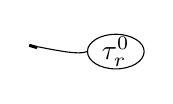
\begin{tikzpicture}[baseline=(z.base),x=1cm,y=1cm]
\node (z) at (.7,0) {$\tau_r^0$};
\draw (.7,0) ellipse (.36 and .22);
\draw (-.4,.08)..controls(-.1,.03)and(.2,-.05)..(.34,0);
\draw[line width=1.1pt](-.4,.08)--(-.3,.05);
\end{tikzpicture}}\\
\gamma_{\pi,s}\\
\gamma'_{\pi,s}\\
\gamma_r^0
\end{array}\\[1em]
\begin{array}{r}\inserted{1020}\\\deleted{\unsure{900}}\end{array} &
\left\{\begin{array}{l}
120=2\times60=1\times120\\
120=2\times60=2\times60\\
120=1\times120=2\times60\\
120=1\times120=2\times60\\
\inserted{3\times}120=\deleted{\unsure{2\times60=2\times60}}\inserted{3\times40=3\times40}\\
120=2\times60=2\times60\\
60=1\times60=2\times30
\end{array}\right. &
\begin{array}{l}
\tau_{\pi,\rho}\\
\gamma_{\pi,\rho}\\
\left.\begin{array}{l}
\unsure{\tau'_r|\tau_r^1}\\
\gamma_r^1\\
\gamma_r^{1'}\\
\gamma_r^2\\
\gamma_r^{2'}
\end{array}\right\}
\end{array}
\end{array}
\]}

\[
\begin{array}{r}
\overline{\overline{\deleted{\unsure{1580|1500}}}}\\
\inserted{1620}
\end{array}
=5\times60+\deleted{\unsure{12}}\inserted{11}\times120
\]

\[
\begin{array}{l}
\tau=\text{``twist''}\\
\gamma=\text{``gommage''}
\end{array}
\]

Programme de travail :

1) déterminer \unsure{les|un} syst. fondamental de
relations entre les \(1620\) flèches
du diagramme, se partageant
\deleted{entre} \(14\) \deleted{\unsure{paquets} de}\inserted{orbites} sous \(\unsure{\mathfrak S_K|\mathfrak G_K}\) (\unsure{aux|avec} \(542\)
sommets, se partageant entre \(9\) orbites)

\margin{en particulier, écrire toutes les flèches comme composés de flèches ``provenant de la dim. modulaire \(\leq1\)''}

\deleted{2) \unsure{Réduire}}

2) Reprendre la question, en éliminant
les sommets du niveau \(0\) (sauf
peut-être ceux de type \(\mathrm I_{10}\) ?),
\deleted{et \(\mathrm{II}_1\) (\unsure{qui} de type \(\mathrm{II}_1\) (qui \unsure{reviennent|revient}
à ceux de type \(\mathrm{III}_1\).) --- mais - Attention
au twist \inserted{\(\mathrm{tw}_{1/6}\)} \unsure{relationnel|relativement} : \(\mathrm{II}_1\) (qui donne
\unsure{un Autom.} de \(=\) type))}

3) Eliminer de plus les pièces
\deleted{\unsure{gauches}} ``tétraédrales'' \(\mathrm{II}_1\) --- et toutes
les pièces qui ne semblent pas
simplifier la présentation des relations.

\figure{\begin{tikzpicture}[x=.006cm,y=-.006cm,line cap=round,line join=round,
ink/.style={draw=black,line width=.6pt},
fine/.style={draw=black,line width=.35pt},
pencil/.style={draw=gray,line width=.35pt},
cut/.style={draw=green!40!black,line width=.8pt,dash pattern=on 1.2pt off 1.3pt},
cutsolid/.style={draw=green!40!black,line width=.8pt}]
% S033 pants
\draw[ink] (2343,133)..controls(2347,181)and(2338,216)..(2317,242);
\draw[ink] (2406,130)..controls(2413,177)and(2430,182)..(2480,180);
\draw[ink] (2482,232)..controls(2428,229)and(2400,244)..(2366,270);
\draw[ink] (2342,129)..controls(2336,117)and(2360,109)..(2380,113)..controls(2402,112)and(2415,118)..(2407,128)..controls(2390,141)and(2354,143)..cycle;
\draw[ink] (2317,242)..controls(2332,231)and(2344,237)..(2356,245)..controls(2370,254)and(2376,266)..(2366,273)..controls(2348,274)and(2328,261)..cycle;
\draw[ink] (2483,180)..controls(2497,176)and(2508,195)..(2504,215)..controls(2502,240)and(2483,243)..(2478,224)..controls(2472,208)and(2476,190)..cycle;
\draw[ink] (2341,239)..controls(2370,210)and(2391,174)..(2411,164)--(2418,170);
\draw[fine,dash pattern=on 1.1pt off 1.3pt] (2369,263)..controls(2397,241)and(2422,210)..(2438,181);
\draw[pencil] (2355,141)..controls(2350,178)and(2351,219)..(2342,240);
\draw[pencil] (2388,142)..controls(2420,172)and(2451,198)..(2481,202);
% S033 four_top
\draw[ink] (2649,129)..controls(2675,142)and(2702,145)..(2720,147);
\draw[ink] (2737,145)..controls(2752,142)and(2765,136)..(2766,131);
\draw[ink] (2798,152)..controls(2794,184)and(2794,213)..(2811,236);
\draw[ink] (2790,270)..controls(2768,233)and(2727,234)..(2684,283);
\draw[ink] (2634,260)..controls(2643,244)and(2649,234)..(2648,225);
\draw[ink] (2648,207)..controls(2652,191)and(2641,162)..(2632,153);
\draw[ink] (2616,149)..controls(2611,140)and(2636,118)..(2646,121)..controls(2660,124)and(2650,145)..(2624,155)..controls(2617,156)and(2615,154)..cycle;
\draw[ink] (2764,131)..controls(2773,115)and(2809,138)..(2807,149)..controls(2806,166)and(2774,152)..cycle;
\draw[ink] (2634,260)..controls(2649,251)and(2678,270)..(2683,284)..controls(2660,289)and(2633,278)..cycle;
\draw[ink] (2810,236)..controls(2819,246)and(2811,269)..(2799,275)..controls(2787,275)and(2786,265)..(2793,253)..controls(2799,243)and(2807,237)..cycle;
\draw[fine,dash pattern=on 1.2pt off 1.4pt] (2648,205)..controls(2699,188)and(2755,187)..(2797,200);
\draw[cut] (2648,205)..controls(2698,190)and(2756,191)..(2797,201);
\draw[fine,dash pattern=on 1.2pt off 1.4pt] (2725,147)..controls(2751,176)and(2741,215)..(2725,244);
\draw[cut] (2728,150)..controls(2752,182)and(2741,219)..(2729,243);
% S033 four_middle
\draw[ink] (2442,359)--(2390,448);
\draw[ink] (2487,361)..controls(2508,372)and(2534,376)..(2543,392)..controls(2546,414)and(2543,440)..(2540,456);
\draw[ink] (2410,468)..controls(2440,465)and(2496,466)..(2517,464);
\draw[ink] (2442,358)..controls(2449,343)and(2476,342)..(2487,356)..controls(2492,374)and(2447,380)..cycle;
\draw[ink] (2390,448)..controls(2397,442)and(2409,446)..(2413,457)..controls(2419,471)and(2408,475)..(2398,469)..controls(2389,463)and(2385,455)..cycle;
\draw[ink] (2521,445)..controls(2532,435)and(2543,444)..(2541,456)..controls(2540,468)and(2524,473)..(2518,460)..controls(2515,453)and(2518,449)..cycle;
\draw[ink] (2533,383)..controls(2544,386)and(2545,398)..(2535,403)..controls(2528,405)and(2526,397)..(2528,390)..cycle;
\draw[fine] (2450,367)--(2451,373) (2458,369)--(2459,374) (2467,369)--(2468,374);
\draw[ink] (2482,372)..controls(2496,395)and(2514,423)..(2530,442);
\draw[ink] (2394,458)--(2408,455);
\draw[fine,dash pattern=on 1.1pt off 1.4pt] (2414,451)..controls(2450,436)and(2492,422)..(2530,404);
\draw[fine,dash pattern=on 1.2pt off 1.3pt] (2408,408)..controls(2450,404)and(2480,409)..(2508,415);
\draw[cut] (2408,408)--(2447,464)--(2508,415)--cycle;
\draw[cut] (2508,415)--(2509,379)--(2543,420)--cycle;
% S033 cancelled_drawing
\draw[fine] (2669,407)--(2666,431);
\draw[ink] (2719,382)--(2730,394)..controls(2750,395)and(2783,407)..(2803,397);
\draw[pencil] (2796,399)..controls(2843,417)and(2838,440)..(2819,451);
\draw[ink] (2819,451)..controls(2804,463)and(2798,471)..(2807,487);
\draw[fine,dash pattern=on 1.3pt off 1.4pt] (2636,477)..controls(2673,449)and(2695,430)..(2750,441)..controls(2786,441)and(2792,455)..(2810,458);
\draw[fine,dash pattern=on 1.3pt off 1.4pt] (2655,499)..controls(2691,490)and(2710,488)..(2739,494);
\draw[fine] (2739,494)--(2787,503);
\draw[cut] (2764,402)..controls(2761,433)and(2750,469)..(2739,494);
\draw[cut] (2661,440)..controls(2714,427)and(2766,439)..(2810,458);
\draw[pencil,line width=.55pt] (2647,443)--(2748,383)--(2668,435)--(2778,385)--(2668,451)--(2787,397)--(2666,465)--(2776,423)--(2666,479)--(2791,430)--(2701,480)--(2802,450)--(2731,487)--(2794,471)--(2744,495)--(2790,483);
% S033 five_holes
\draw[ink] (2370,565)..controls(2356,599)and(2335,622)..(2296,632);
\draw[ink] (2450,570)..controls(2463,620)and(2485,642)..(2522,645);
\draw[ink] (2522,698)..controls(2487,725)and(2491,760)..(2493,787);
\draw[ink] (2458,812)..controls(2418,789)and(2386,799)..(2353,807);
\draw[ink] (2310,788)..controls(2315,736)and(2300,706)..(2276,683);
\draw[ink] (2370,565)..controls(2375,553)and(2437,551)..(2450,563)..controls(2458,579)and(2383,585)..cycle;
\draw[ink] (2296,632)..controls(2276,627)and(2265,666)..(2276,683)..controls(2295,681)and(2312,642)..cycle;
\draw[ink] (2522,645)..controls(2538,652)and(2540,692)..(2522,701)..controls(2510,697)and(2507,654)..cycle;
\draw[ink] (2310,788)..controls(2328,783)and(2360,798)..(2353,809)..controls(2338,822)and(2299,805)..cycle;
\draw[ink] (2493,787)..controls(2505,798)and(2494,813)..(2474,816)..controls(2457,819)and(2450,808)..(2464,798)..controls(2478,788)and(2487,785)..cycle;
\draw[cut] (2357,588)..controls(2394,631)and(2455,690)..(2507,706);
\draw[cut] (2317,621)..controls(2347,640)and(2355,676)..(2366,720);
\draw[cutsolid] (2366,720)..controls(2372,748)and(2393,775)..(2387,803);
\draw[cut] (2300,692)..controls(2340,659)and(2411,627)..(2460,604);
\draw[cut] (2478,642)..controls(2464,684)and(2449,707)..(2445,728);
\draw[cutsolid] (2443,736)..controls(2442,764)and(2437,781)..(2436,797);
\draw[cut] (2315,746)..controls(2336,738)and(2353,729)..(2363,726);
\draw[cutsolid] (2382,727)..controls(2403,727)and(2434,729)..(2443,736);
\draw[cut] (2454,738)..controls(2470,739)and(2478,744)..(2482,749);
\draw[pencil] (2296,632)..controls(2338,589)and(2362,558)..(2410,558)..controls(2470,561)and(2504,601)..(2516,646);
\draw[pencil] (2276,683)..controls(2276,748)and(2278,778)..(2310,788);
\draw[pencil] (2308,650)..controls(2380,638)and(2429,615)..(2460,604);
\draw[pencil] (2356,655)..controls(2411,641)and(2430,637)..(2478,642);
\draw[pencil] (2386,803)..controls(2410,781)and(2428,796)..(2463,811);
% S033 sphere_left
\draw[ink] (2259,980)..controls(2222,1010)and(2146,1022)..(2134,1117)..controls(2123,1190)and(2159,1226)..(2252,1249)..controls(2262,1253)and(2262,1264)..(2266,1268);
\draw[ink] (2338,982)..controls(2366,1015)and(2429,1017)..(2441,1093)..controls(2454,1194)and(2417,1230)..(2342,1251)..controls(2331,1260)and(2340,1267)..(2327,1270);
\draw[ink] (2259,977)..controls(2252,963)and(2329,960)..(2338,975)..controls(2343,988)and(2266,991)..cycle;
\draw[ink] (2266,1268)..controls(2284,1278)and(2314,1276)..(2327,1270);
\draw[fine,dash pattern=on 1.3pt off 1.3pt] (2267,1256)..controls(2279,1244)and(2318,1244)..(2332,1254);
\draw[ink] (2174,1141)..controls(2175,1113)and(2210,1110)..(2233,1140)..controls(2246,1168)and(2226,1191)..(2198,1183)..controls(2176,1179)and(2167,1162)..cycle;
\draw[ink] (2366,1146)..controls(2356,1120)and(2387,1102)..(2406,1115)..controls(2431,1133)and(2423,1166)..(2401,1174)..controls(2379,1182)and(2363,1171)..cycle;
\draw[fine,dash pattern=on 1.4pt off .7pt] (2261,1093)..controls(2262,1071)and(2288,1055)..(2309,1062)..controls(2328,1071)and(2338,1114)..(2319,1120)..controls(2297,1134)and(2261,1124)..cycle;
\draw[ink] (2132,1130)..controls(2143,1142)and(2160,1144)..(2172,1151);
\draw[ink] (2238,1157)..controls(2277,1166)and(2326,1162)..(2365,1152);
\draw[ink] (2423,1139)..controls(2432,1135)and(2437,1128)..(2442,1125);
\draw[fine,dash pattern=on .8pt off 1.1pt] (2135,1113)..controls(2176,1094)and(2219,1095)..(2261,1093);
\draw[fine,dash pattern=on 1.4pt off .8pt] (2330,1093)..controls(2369,1098)and(2405,1092)..(2442,1116);
\draw[pencil] (2250,992)..controls(2243,1048)and(2254,1115)..(2243,1173)..controls(2237,1216)and(2235,1230)..(2246,1248);
\draw[pencil] (2348,994)..controls(2357,1034)and(2328,1087)..(2340,1134)..controls(2346,1177)and(2370,1210)..(2351,1255);
\draw[pencil,line width=.5pt] (2155,1048)..controls(2190,1050)and(2232,1090)..(2267,1128)..controls(2306,1179)and(2335,1228)..(2351,1255);
\draw[pencil,dash pattern=on 1.1pt off 1.1pt] (2155,1048)..controls(2173,1101)and(2225,1155)..(2269,1202)..controls(2300,1230)and(2324,1243)..(2344,1255);
\draw[pencil,dash pattern=on 1pt off 1.1pt] (2245,1249)..controls(2273,1224)and(2302,1230)..(2346,1252);
\draw[pencil] (2243,1087)..controls(2240,1049)and(2317,1031)..(2400,1035)..controls(2444,1032)and(2442,1081)..(2422,1088);
\draw[pencil] (2330,1092)..controls(2365,1095)and(2401,1099)..(2422,1088);
\draw[pencil] (2357,1148)..controls(2351,1108)and(2395,1106)..(2426,1121)..controls(2449,1161)and(2426,1211)..(2387,1208)..controls(2355,1207)and(2348,1173)..cycle;
\draw[pencil] (2364,1145)..controls(2360,1118)and(2399,1114)..(2422,1131);
\draw[pencil] (2383,1126)..controls(2417,1127)and(2431,1148)..(2403,1143);
\draw[fine] (2132,1135)..controls(2129,1144)and(2133,1154)..(2127,1165)--(2134,1159);
% S033 sphere_right
\draw[ink] (2701,990)..controls(2686,1021)and(2595,1034)..(2564,1115)..controls(2547,1190)and(2590,1275)..(2668,1301)..controls(2730,1325)and(2854,1304)..(2880,1239)..controls(2916,1160)and(2913,1081)..(2878,1048)..controls(2854,1028)and(2816,1021)..(2810,997);
\draw[ink] (2701,986)..controls(2724,966)and(2785,976)..(2810,990)..controls(2825,1007)and(2736,1008)..cycle;
\draw[pencil] (2703,985)..controls(2735,980)and(2782,988)..(2805,999);
\draw[ink] (2619,1172)..controls(2611,1144)and(2642,1132)..(2664,1156)..controls(2688,1182)and(2660,1219)..(2635,1211)..controls(2622,1206)and(2616,1187)..cycle;
\draw[fine,line width=.6pt] (2813,1181)..controls(2817,1155)and(2841,1156)..(2856,1185)..controls(2872,1220)and(2846,1231)..(2825,1219)..controls(2812,1210)and(2810,1198)..cycle;
\draw[fine,dash pattern=on 1.3pt off .9pt] (2653,1105)..controls(2648,1084)and(2677,1075)..(2692,1092)..controls(2710,1115)and(2690,1146)..(2669,1138)..controls(2652,1133)and(2646,1120)..cycle;
\draw[fine,dash pattern=on 1.5pt off .6pt] (2824,1112)..controls(2816,1091)and(2842,1093)..(2860,1106)..controls(2882,1123)and(2867,1152)..(2844,1144)..controls(2826,1144)and(2820,1129)..cycle;
\draw[ink] (2564,1146)..controls(2572,1158)and(2598,1164)..(2618,1169);
\draw[ink] (2673,1190)..controls(2728,1190)and(2778,1202)..(2814,1198);
\draw[ink] (2860,1193)..controls(2880,1173)and(2887,1176)..(2898,1161);
\draw[fine,dash pattern=on 1.5pt off .9pt] (2568,1132)..controls(2597,1115)and(2629,1118)..(2651,1109);
\draw[fine] (2695,1104)..controls(2708,1110)and(2724,1111)..(2736,1111);
\draw[fine,dash pattern=on 1.4pt off 1pt] (2754,1111)..controls(2780,1115)and(2803,1117)..(2822,1112);
\draw[fine] (2870,1130)..controls(2884,1130)and(2895,1139)..(2900,1142);
\draw[pencil,line width=.65pt] (2669,1028)..controls(2629,1069)and(2597,1135)..(2596,1200)..controls(2599,1260)and(2635,1270)..(2670,1234)..controls(2728,1170)and(2775,1073)..(2809,1020);
\draw[pencil,line width=.6pt] (2812,1022)..controls(2778,1093)and(2744,1163)..(2675,1237);
\draw[pencil] (2671,1026)..controls(2663,1079)and(2661,1154)..(2674,1237)..controls(2684,1277)and(2701,1300)..(2714,1308);
\draw[pencil,dash pattern=on 1.4pt off 1.1pt] (2673,1024)..controls(2722,1037)and(2723,1104)..(2729,1176)..controls(2730,1257)and(2725,1289)..(2714,1308);
\draw[pencil,line width=.5pt] (2816,1021)..controls(2808,1072)and(2785,1142)..(2770,1214)..controls(2764,1263)and(2751,1301)..(2758,1309);
\draw[pencil,dash pattern=on 1.4pt off 1.2pt] (2820,1027)..controls(2830,1092)and(2809,1170)..(2795,1243)..controls(2784,1285)and(2769,1302)..(2758,1309);
\draw[fine,line width=.65pt] (2745,1310)--(2715,1310)--(2737,1320);
\draw[fine,line width=.65pt] (2783,1304)--(2808,1296)--(2796,1308);
% S033 isolated_arc
\draw[pencil] (1978,699)..controls(1976,753)and(2037,766)..(2056,724);
% S033 grouping
\draw[pencil] (2309,139)..controls(2279,178)and(2264,271)..(2304,298)..controls(2379,315)and(2497,283)..(2561,210)..controls(2612,157)and(2605,118)..(2615,82);
\draw[pencil] (2615,82)..controls(2653,40)and(2674,27)..(2710,18);
\draw[pencil] (2770,20)..controls(2843,58)and(2926,134)..(2898,217)..controls(2862,326)and(2767,392)..(2647,455)..controls(2538,514)and(2416,540)..(2361,498)..controls(2321,465)and(2319,403)..(2352,365);
\draw[pencil] (2154,854)..controls(2205,703)and(2244,570)..(2322,532)..controls(2408,498)and(2569,512)..(2642,564)..controls(2701,608)and(2713,758)..(2768,808)..controls(2855,871)and(2915,1014)..(2919,1161)..controls(2916,1312)and(2909,1375)..(2812,1379)..controls(2669,1376)and(2556,1364)..(2456,1374)..controls(2303,1385)and(2133,1356)..(2084,1306)..controls(2029,1247)and(2048,1086)..(2079,977)..controls(2098,920)and(2135,897)..(2154,854);
\draw[pencil] (1950,1406)..controls(1978,1421)and(2014,1410)..(2059,1414)--(2855,1418);
% S033 large_surface
\draw[pencil] (2048,1682)..controls(1996,1624)and(2047,1571)..(2168,1504)..controls(2211,1479)and(2250,1473)..(2276,1491)..controls(2314,1540)and(2249,1631)..(2168,1672)..controls(2109,1701)and(2055,1707)..(2048,1682);
\draw[fine,line width=.55pt] (2276,1491)..controls(2302,1534)and(2264,1597)..(2227,1635)..controls(2178,1673)and(2098,1709)..(2048,1682);
\draw[pencil] (2044,1685)..controls(2124,1717)and(2246,1660)..(2288,1570)..controls(2305,1530)and(2292,1504)..(2276,1491);
\foreach \x/\y in {2276/1491,2257/1600,2168/1672,2048/1682,2069/1585,2168/1504}{
\draw[fine,line width=.7pt] (\x-8,\y)--(\x+8,\y) (\x-5,\y-7)--(\x+5,\y+7) (\x-5,\y+7)--(\x+5,\y-7);
}
\foreach \x/\y in {2285/1549,2227/1635,2110/1690,2048/1627,2110/1543,2218/1485}{\fill (\x,\y) circle[radius=.7pt];}
\draw[fine,line width=.6pt] (2284,1517)--(2296,1512)
(2261,1573)--(2289,1584)
(2241,1613)--(2249,1618)
(2196,1648)--(2204,1655)
(2137,1671)--(2148,1694)
(2080,1688)--(2080,1697)
(2035,1652)--(2043,1652)
(2047,1603)--(2069,1612)
(2085,1561)--(2094,1567)
(2132,1522)--(2138,1528)
(2185,1487)--(2193,1504)
(2246,1478)--(2246,1486);
\draw[fine] (2048,1682)..controls(2091,1781)and(2164,1879)..(2154,1982)..controls(2156,2084)and(2068,2184)..(2019,2219);
\draw[pencil] (2048,1682)..controls(2108,1802)and(2182,1889)..(2174,1987)..controls(2156,2064)and(2076,2111)..(2003,2154);
\draw[pencil] (2048,1682)..controls(2070,1734)and(2090,1752)..(2115,1775);
\draw[fine] (2276,1491)..controls(2340,1613)and(2472,1700)..(2575,1745)..controls(2701,1793)and(2855,1734)..(2968,1721)..controls(2980,1717)and(2989,1723)..(2995,1731);
\draw[pencil] (2281,1505)..controls(2334,1620)and(2499,1704)..(2583,1741)..controls(2719,1773)and(2856,1724)..(2963,1719);
\draw[pencil] (2291,1518)..controls(2338,1582)and(2401,1634)..(2489,1677);
\draw[pencil] (2973,1727)..controls(2940,1802)and(2924,1949)..(2936,2026)..controls(2939,2050)and(2952,2057)..(2962,2064);
\draw[fine] (2962,1734)..controls(2930,1812)and(2920,1944)..(2927,2017)..controls(2931,2043)and(2950,2060)..(2961,2066);
\draw[pencil] (2980,1733)..controls(2963,1805)and(2964,1899)..(2970,1938);
\draw[pencil] (2955,2071)..controls(2823,2099)and(2721,2150)..(2630,2217);
\draw[pencil] (2949,2066)..controls(2818,2097)and(2688,2160)..(2625,2228);
\draw[pencil] (2940,2051)..controls(2897,2050)and(2847,2083)..(2821,2102);
\draw[pencil] (2019,2219)..controls(2015,2201)and(2058,2209)..(2080,2228);
\end{tikzpicture}}

\margin{32}
